This section presents the main results of the paper. First, it shows that \emph{Plan Cuadrante} significantly improved crime and crime perception outcomes. Second, it shows that these effects were consistent across municipalities with different population densities and with varying socioeconomic levels. Finally, the section studies which components of the program are driving the effects. 

\subsection{Effects of \emph{Plan Cuadrante} on Crime and Security Perception}
\label{main_results}

Panels (a) to (d) in Figure \ref{fig:figure02} present estimates of the dynamic effects of \emph{Plan Cuadrante} on victimization, reported crime, crime perception, and investment in household security measures. The blue circles and bars represent pre-adoption estimates and their 95\% confidence intervals. Very few of these pre-treatment coefficients are statistically significant, and the average pre-treatment effects are overall reassuring,\footnote{The p-values for the test that the average pre-treatment effect equals zero are 0.833 for victimization, 0.204 for reported crime, 0.178 for security perception, and 0.066 for the adoption of security measures.} suggesting that the outcomes that we study followed parallel trends before the program's introduction.%The p-values for the \emph{joint} significance test of the pre-treatment coefficients are, respectively, 0.101, 0.049, 0.076, and 0.109. The only marginal case is the joint test for reported crime, where the pre-treatment coefficients are slightly positive and therefore conservative with respect to the negative effect we estimate.0.159 for arrests, 0.300 for trust in police 
 

\FloatBarrier
%--- Implementation
\begin{figure}[h!]
    \centering
    \caption{Effects of \emph{Plan Cuadrante} on Crime Outcomes and Security Perceptions}
    \label{fig:figure02}
    \begin{subfigure}{0.495\textwidth}
        \centering
        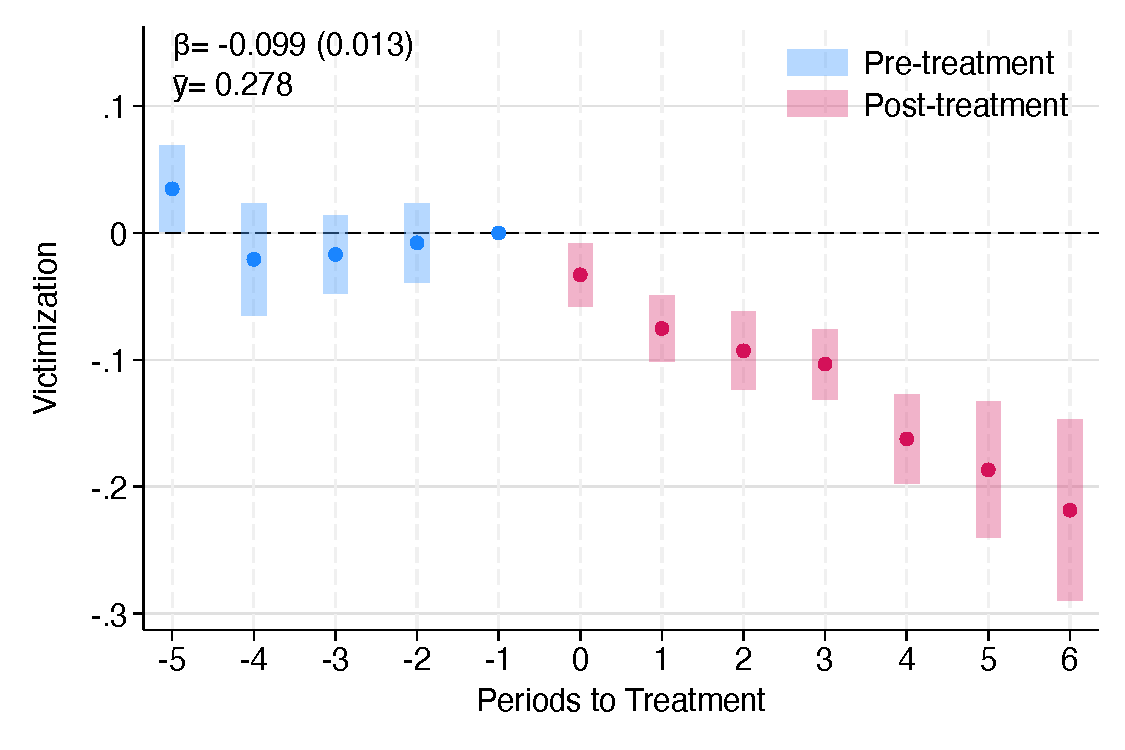
\includegraphics[width=\textwidth]{../manuscript/Graphs/results_victimization.pdf}
        \caption{Victimization in last 12 months}
    \end{subfigure}%
    ~
    \begin{subfigure}{0.495\textwidth}
    \centering
    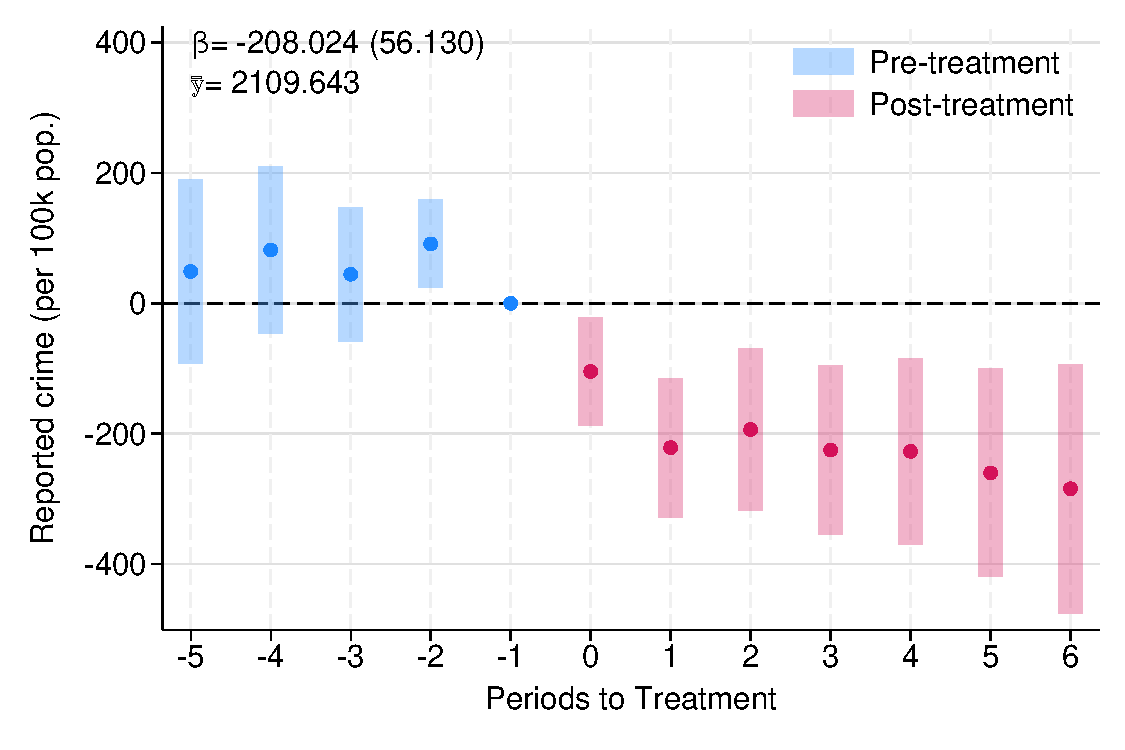
\includegraphics[width=\textwidth]{../manuscript/Graphs/totalreportedcrime_allcomunas.pdf}
        \caption{Reported crime per 100k inhabitants}
    \end{subfigure}
        \begin{subfigure}{0.495\textwidth}
        \centering
        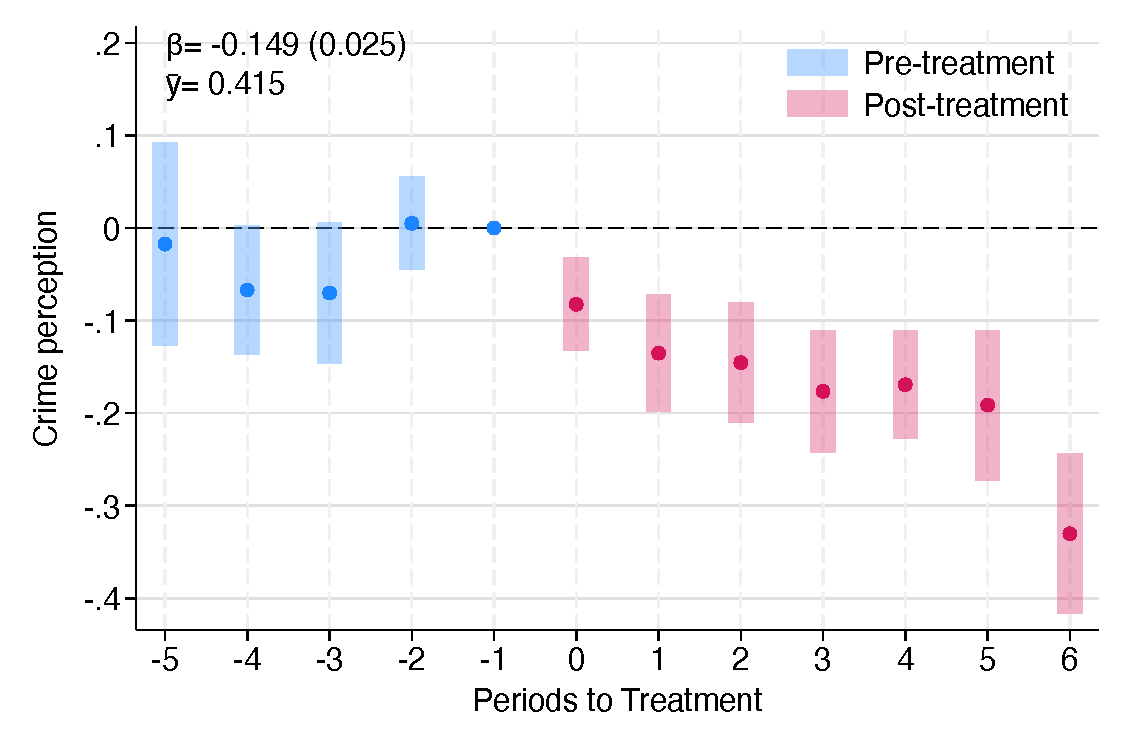
\includegraphics[width=\textwidth]{../manuscript/Graphs/results_perception.pdf}
        \caption{Households reporting an increase in crime}
    \end{subfigure}%
    ~
    \begin{subfigure}{0.495\textwidth}
    \centering
    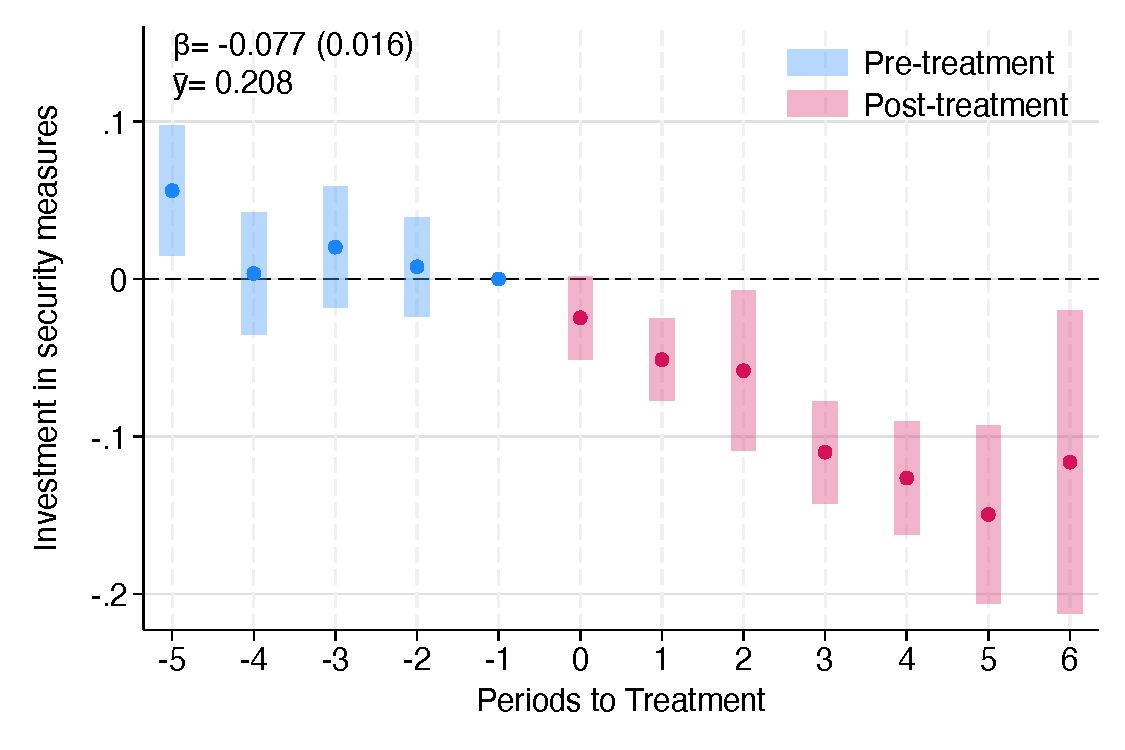
\includegraphics[width=\textwidth]{../manuscript/Graphs/results_hhprotectionmeasures.pdf}
        \caption{Households adopting security measures}
    \end{subfigure}
    \\[12pt]
    \begin{minipage}{0.99\textwidth}
    \footnotesize
    Notes: This figure shows the dynamic effects of the \emph{Plan Cuadrante} on different measures of police effectiveness. The estimation is conducted using the procedure developed in \citet{Callaway} for difference-in-differences with staggered treatment adoption. The dots in the figure represent the estimated coefficients and the bars behind them 95\% confidence intervals. Standard errors are clustered at the municipality level using the wild bootstrapping procedure. The pooled effect and the mean outcome before the introduction of the treatment is also presented in each panel. Panel (a) reports the effect of \emph{Plan Cuadrante} on the probability of household victimization in the last 12 months using the ENUSC survey. Panel (b) reports the effect on the number of crimes reported to the police in the municipality per 100,000 inhabitants using administrative data. Panel (c) reports the effect on the probability of perceiving an increase in crime using the ENUSC survey. Panel (d) reports the effect on the probability of adopting security measures in the last twelve months using the ENUSC survey. Panel (a) includes 93,041 observations; panel (b), 4,231; panel (c), 89,578; and panel (d), 93,041 observations.
    \end{minipage}
\end{figure}

\FloatBarrier

The red circles and bars represent post-adoption estimates and illustrate the program's effects.\footnote{The analyses we present in this section come from an unbalanced panel of municipalities. Thus, each lead and lag is identified using a different subset of municipalities. Online Appendix Figure \ref{fig:figureA6_bp} replicates these analyses using only municipalities that implemented \emph{Plan Cuadrante} between 2006 and 2009, allowing us to build a balanced panel between t-2 and t+3. The estimates remain remarkably similar.}

Panel (a) shows that after adopting \emph{Plan Cuadrante}, there was a significant drop in the share of households reporting crimes in the previous 12 months. This decline in victimization begins in the adoption year and continues over time, falling by ten percentage points (36\%) on average. Consistently, panel (b) shows a substantial decrease in reported crimes. Expressed per hundred thousand inhabitants to normalize across municipality sizes, we find an average reduction of 208 reported crimes (10\%) following the adoption of the program.\footnote{Table \ref{tab:bonferroni} in Online Appendix \ref{sec:appendixC} applies the Bonferroni correction across the main outcome estimates and confirms that these results are not a product of multiple hypothesis testing.}\footnote{For symmetry with the ENUSC-based analysis, this event study is restricted to 5 pre-treatment and 7 post-treatment periods. Since the administrative data cover a much larger number of never-treated municipalities than the ENUSC sample, we can estimate this effect over a longer window of pre-treatment and post-treatment periods; Online Appendix Figure \ref{fig:admin_uncapped} reports the results for reported crime and arrests using the full set of post-treatment and pre-treatment periods, which are very similar to those presented here.}\footnote{Online Appendix Figure \ref{fig:figureA9} reports a placebo exercise confirming the absence of effects on crimes that we would not expect to respond to \emph{Plan Cuadrante}.}\footnote{As a further robustness check, we implement a placebo/randomization-inference exercise in which adoption dates and never-treated status are randomly reassigned 1,000 times: our estimated direct effect on treated municipalities falls in the bottom first percentile of the resulting placebo distribution, while the analogous estimate for untreated neighbors of treated municipalities falls near its center---consistent with a genuine effect on treated municipalities and with the absence of spillovers documented in Section \ref{sec:spillovers} (Online Appendix \ref{sec:ri_appendix}).} Note, however, that analyses based on reported cases may underestimate the reform's true impact since not all crimes are reported to the police.\footnote{Online Appendix Figure \ref{fig:figureA8} replicates the analyses in panels (a) and (b) by crime type, showing significant reductions in both property and violent crimes. While the definitions of crime categories differ across survey and administrative data, the program's effects are consistent in magnitude and statistical significance for violent theft, assault, and home burglary in both datasets.}
%, and improved trust in police could increase reporting rates, making any observed reductions in reported crime a conservative estimate of the actual crime decline.
%Panel (c) shows that despite the decrease in victimization and reported crime, arrests per hundred thousand inhabitants increased following the adoption of \emph{Plan Cuadrante}. This simultaneous decrease in crimes and increase in arrests suggests improved police effectiveness.

The results above show that \emph{Plan Cuadrante} reduced both victimization and reported crime. But did this change in public safety translate into increased security perception? Panel (c) reveals that \emph{Plan Cuadrante} decreased insecurity perception, with households reporting increased neighborhood crime dropping by 15 percentage points (36\%).\footnote{Online Appendix Figure \ref{fig:figureA3} reports similar declines in insecurity perception measured at the municipality and country levels.} In line with this result, panel (d) shows that following the program implementation, households adopting protective measures---such as buying dogs or weapons, installing alarms or fences, and purchasing insurance or private security---decreased by eight percentage points (37\%).\footnote{Online Appendix Table \ref{tab:hhprotectionmeasurestype} disaggregates this analysis by measure type.}
%Panel (d) shows that households reporting high or very high trust in police increased by 12 percentage points (30\%) in adopting municipalities. 

In sum, \emph{Plan Cuadrante} reduced both criminal activity and security perception, while also decreasing private investment in security measures.\footnote{These results are robust to excluding municipalities most affected by the 2010 Maule earthquake, defined as those with a Modified Mercalli Intensity greater than 7; see Figure \ref{fig:figure02_noEQ} in Online Appendix \ref{sec:appendixC} for details.}

%To benchmark the scale of these effects in more intuitive terms, we translate the estimated decline in victimization into the number of victims avoided. Using the average annual cost of the program per municipality---US\$3.47 million \citep{DIPRES2007_largo, DIPRES2014}---and the 2017 Census total population across the 150 municipalities that adopted \emph{Plan Cuadrante}---15,424,263 inhabitants \citep{INE2017_censo}---the implied cost per victim avoided is about US\$338. Because beat policing is essentially a reorganization of police deployment, municipalities or police departments that are already well staffed and equipped would face substantially lower implementation costs. Overall, the cost of \emph{Plan Cuadrante} compares favorably with the substantial social and economic costs that crime imposes on households and communities in Latin America \citep{jaitman2017costs}.


%each percentage-point increase in trust in the police costs approximately US\$289,000, and  and each additional arrest per 100,000 inhabitants approximately US\$72,000

\subsection{\emph{Plan Cuadrante} and Spatial Spillovers}
\label{sec:spillovers}
%\textbf{4.2 \emph{Plan Cuadrante} and Spatial Spillovers}

Beyond parallel trends, a causal interpretation of our estimates requires the absence of spillover effects from treated to control municipalities, since such spillovers could bias treatment effects upward. This concern is relevant in our setting. Previous work on deployment-based policing reforms, such as hot-spot policing, shows that crime may be displaced to nearby areas \citep{Blattman_Tobon_JEEA}. Spillovers could also arise through the reallocation of police resources from control to treated municipalities.

In our setting, spillovers are less likely for several reasons. First, as discussed in Section \ref{institutions}, \emph{Plan Cuadrante} introduced beat policing in Chile by reorganizing deployment across the full municipal territory rather than concentrating resources in specific hot spots. Second, Chilean municipalities are large---on average 101,000 inhabitants and 2,000 square kilometers \citep{SINIM}---and criminals typically do not travel such long distances to commit crimes, which makes displacement to other municipalities unlikely \citep{Langella}. Third, and more directly related to police resources, police regulations assign officers to \emph{comisar\'ias}---broader operational units that usually cover an entire municipality---for fixed periods, which limits rapid reallocation of officers across jurisdictions.\footnote{See the Transfer Manual for Carabineros de Chile Personnel available at \url{https://www.carabineros.cl/transparencia/og/pdf/OG_2707_13112019.pdf}}

We nonetheless assess spillovers empirically through two complementary exercises using administrative data at the national level. Online Appendix \ref{sec:appendixC} reports the full results. First, following \citet{crepon2013}, we test whether higher exposure to \emph{Plan Cuadrante} among neighboring municipalities affects outcomes in control municipalities. Online Appendix Figures \ref{fig:figure_continuous_spillovers} and \ref{fig:figure_count_spillovers}---which define neighbor exposure as the share and the number of treated neighbors, respectively---show no meaningful effects across the outcomes we study, suggesting the absence of spatial spillovers. Because exposure to treated neighbors is not randomly assigned, however, this evidence does not fully rule out the possibility that municipalities with many early-adopting neighbors differ systematically from those with fewer such neighbors in other respects that are also correlated with our outcomes.

Second, we estimate the effect of \emph{Plan Cuadrante} on police-reported crime and police resources in untreated municipalities whose neighbors adopt the program. Online Appendix Figure \ref{fig:spillover_admin} summarizes these estimates and again shows no evidence of spatial spillovers.

The exercises above evaluate spatial spillovers using administrative records for the extended municipality sample. We complement this evidence with two additional analyses focused on ENUSC municipalities. First, we re-estimate the administrative-outcome spillover analysis---for reported crime, arrests, police officers, and patrol vehicles---restricting the sample to neighbors of the 46 ENUSC municipalities (Online Appendix Figure \ref{fig:figure_46ENUSC_spillovers_admin}). Second, we test for spillovers directly in ENUSC outcomes. Because ENUSC coverage is limited---46 treated municipalities and 1 never-treated municipality, with only 10 sharing a border and 6 of those treated in different years---we estimate spillover effects from early-adopting ENUSC municipalities onto late-adopting ENUSC neighbors before the latter adopt the program (Online Appendix Figure \ref{fig:figure_results_spillovers_enusc}). Both exercises yield reassuringly null effects.

Taken together, these results indicate that spatial spillovers are unlikely to threaten identification in our setting.

\FloatBarrier

\subsection{Heterogeneous Effects of \emph{Plan Cuadrante} by Municipality and Households Characteristics}
\label{heterogeneity}

This section examines whether \emph{Plan Cuadrante}'s effects vary by population density, municipal poverty rates, and household socioeconomic status.\footnote{Data on population density and municipal poverty rates are available at \url{https://www.sinim.gov.cl/}} These analyses inform both external validity and distributional effects of the program. Figure \ref{fig:figure04_het} summarizes these results. We compare municipalities with low versus high population density, municipalities with low versus high poverty rates, and households with low versus high socioeconomic status by splitting the sample in two and estimating specification (\ref{eq:main}) independently in each subsample. For each split, we study four outcomes: victimization, reported crime, crime perception, and investment in security measures. Panels (a) and (b) plot victimization, crime perception, and investment in security measures---from the National Survey on Security and Crime (ENUSC)---on the left axis, and reported crime---from the administrative data of the Undersecretary for Crime Prevention---on the right axis. Because socioeconomic status is only observed in the ENUSC, panel (c) reports the three survey-based outcomes only. Blue and red bars represent $\beta_1$ estimates from different subsamples.

\FloatBarrier
%--- Implementation
\begin{figure}[h!]
    \centering
    \caption{Effects of \emph{Plan Cuadrante} by Population Density, Poverty, and Socioeconomic Status}
    \label{fig:figure04_het}
    \begin{subfigure}[t]{0.49\textwidth}
        \centering
        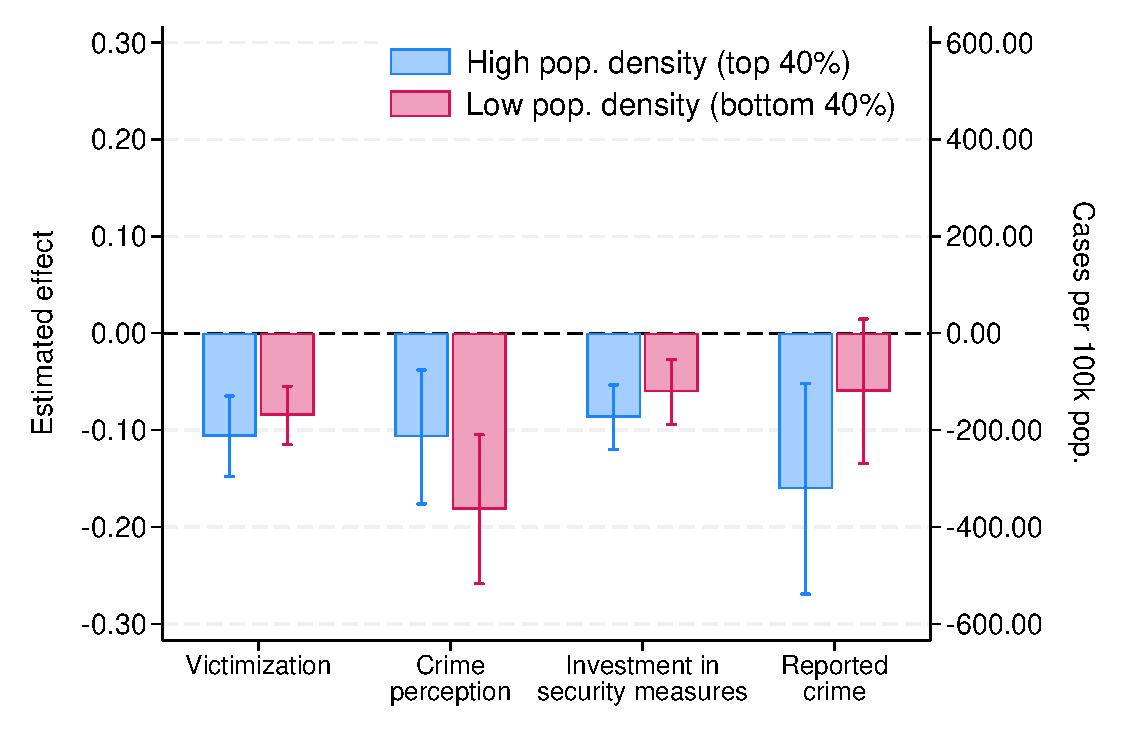
\includegraphics[width=\linewidth]{../manuscript/Graphs/results_het_density.pdf}
        \caption{By population density}
    \end{subfigure}\hfill
    \begin{subfigure}[t]{0.49\textwidth}
        \centering
        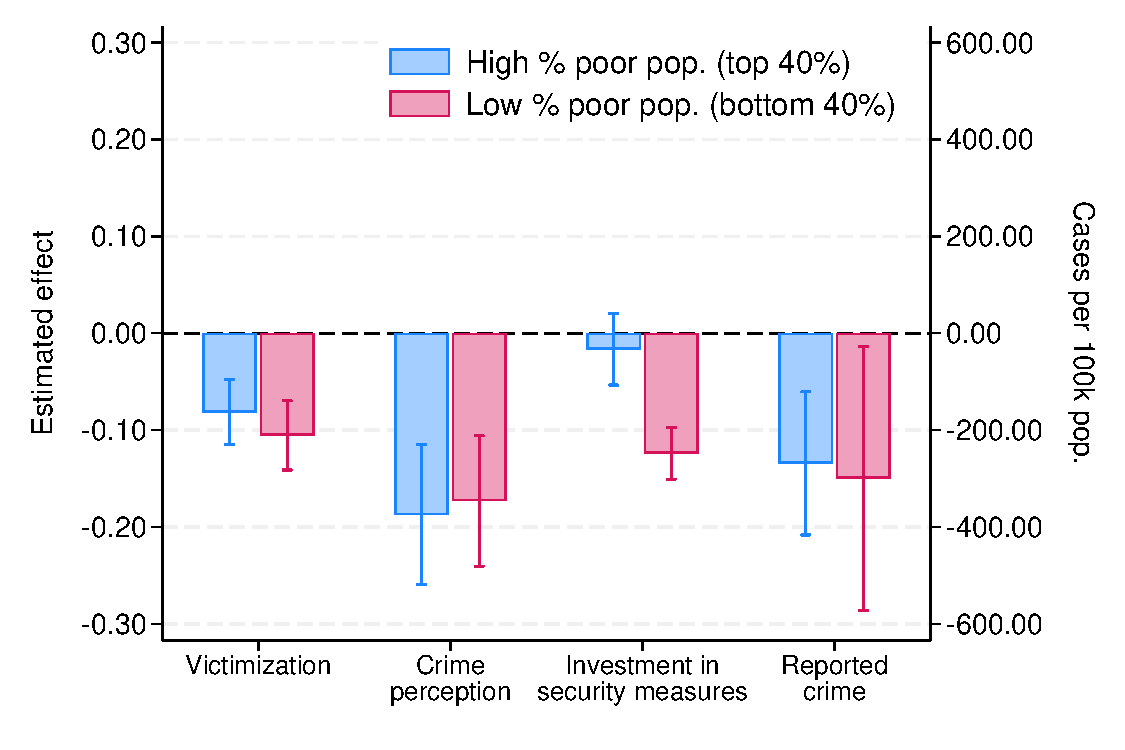
\includegraphics[width=\linewidth]{../manuscript/Graphs/results_het_poorpop.pdf}
        \caption{By population below poverty line}
    \end{subfigure}
    \\[8pt]
    \begin{subfigure}[t]{0.49\textwidth}
        \centering
        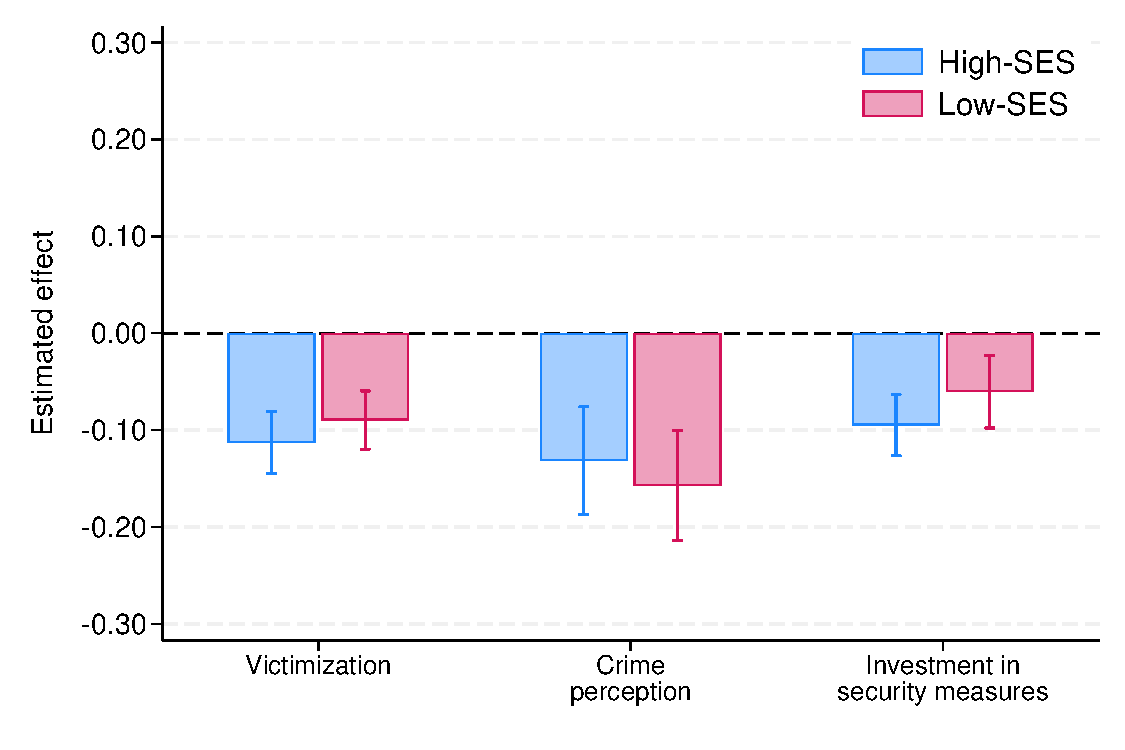
\includegraphics[width=\linewidth]{../manuscript/Graphs/results_het_SES.pdf}
        \caption{By household socioeconomic status}
    \end{subfigure}
    \\[10pt]
    \begin{minipage}{0.99\textwidth}
    \footnotesize Notes: This figure reports the heterogeneous effects of \emph{Plan Cuadrante} by population density (panel a), the proportion of poor people in the municipality (panel b), and household socioeconomic status (panel c). Each panel reports the effect on victimization, defined as the probability of household victimization in the last 12 months; crime perception, defined as the probability of perceiving an increase in crime; investment in security measures, defined as the probability of adopting security measures in the last twelve months; and reported crime, defined as the number of crimes reported to the police in the municipality per 100,000 inhabitants. Reported crime (administrative data, in cases per 100,000 inhabitants) is read on the right axis; all other outcomes, from the ENUSC survey (victimization, crime perception, and investment in security measures), are read on the left axis. Household socioeconomic status is only observed in the ENUSC, so panel (c) does not include reported crime. In panels (a) and (b), the bars compare municipalities in the two bottom quintiles (bottom 40\%) and in the two top quintiles (top 40\%) of the population density and poverty distributions, respectively. The average population density is 458 inhabitants per square kilometer in high-density municipalities and 29 in low-density municipalities; the average poverty rate is 28\% in high-poverty municipalities and 14\% in low-poverty municipalities. In panel (c), low-SES households include lower-class and lower-middle-class households, while high-SES households include upper-middle and upper-class households. The estimation is conducted using the difference-in-differences estimator for staggered treatment adoption developed in \citet{Callaway}. The graphs display the estimated coefficients and 95\% confidence intervals. Standard errors are clustered at the municipality level using the wild bootstrapping procedure.
    \end{minipage}
\end{figure}

\FloatBarrier

While \emph{Plan Cuadrante} was implemented only in urban municipalities, these areas vary substantially in size and structure. Yet panel (a) shows similar effects across population densities. Blue bars illustrate effects in high-density municipalities---top 40\% of density distribution---and red bars in low-density municipalities---bottom 40\%.\footnote{Average density: 458 inhabitants per square kilometer in high-density municipalities versus 29 in low-density municipalities.}

Panel (b) presents the results of a similar exercise comparing municipalities with different poverty rates. As in the case of population density, effects of \emph{Plan Cuadrante} seem to be similar across municipalities with high- and low-poverty rates. Blue bars show effects in high-poverty municipalities---top 40\% of poverty rate distribution---and red bars in low-poverty municipalities---bottom 40\%.\footnote{Average poverty rate: 28\% in high-poverty municipalities versus 14\% in low-poverty municipalities.}

Finally, panel (c) indicates that effects on victimization and security perception do not vary across household socioeconomic status (SES), based on ENUSC's household self-reported classification.\footnote{SES classification: Low-SES includes lower-class and lower-middle-class households; high-SES includes upper-middle and upper-class households.} Blue bars represent high-SES households, red bars low-SES households.

These results indicate that the beat policing model induced by \emph{Plan Cuadrante} benefited municipalities and households similarly, regardless of population density or socioeconomic status.

%% DANI, las figuras de heterogeneidad tienen que enfocarse exclusivamente en los outcomes de victimización, reported crime, percepción de inseguriad y adopción de medidas de seguridad. No hemos introducido los resultados de confianza en la policía y arrestos aún, por lo que sería raro que aparezcan acá.

\subsection{What Is Driving the Effects of \emph{Plan Cuadrante}?}%
\label{mechanisms}
%\textbf{4.4 What Is Driving the Effects of \emph{Plan Cuadrante}?}


To reduce crime and improve security perceptions, police forces need to strengthen both prevention and police effectiveness. Both margins can be shaped by resources, territorial deployment, and policing strategy. This section examines which components of \emph{Plan Cuadrante} are most likely to drive the effects documented in Section \ref{results}. 

The central objective of \emph{Plan Cuadrante} was to introduce a beat policing model by reorganizing deployment. Police operational territories that had typically matched municipal boundaries were subdivided into quadrants, and officers were permanently assigned to these quadrants. During our study period, national operational guidelines remained the same in adopting and non-adopting municipalities. Still, this new deployment likely affected policing strategy at a more operational level, because it allowed officers to adapt patrol routes, schedules, and prevention practices using the local knowledge that the program sought to build.

Although changes in resources were not the core of the reform, implementation contemplated increases in municipalities that lacked the personnel and patrol capacity required to move to this model. During the period we study, Chile was expanding public spending on security, and police resources increased in most municipalities regardless of whether or when they adopted \emph{Plan Cuadrante}. On average, however, municipalities adopting the program experienced larger increases in officers and patrol vehicles, as shown in panels (a) and (b) of Figure \ref{fig:resources}. Since increases in police resources have been shown to reduce crime in some contexts \citep{Evans}, this pattern raises a central question for interpretation, namely whether our estimates reflect resource expansion or the deployment and strategy changes introduced by \emph{Plan Cuadrante}. We address this question through a set of exercises that exploit heterogeneity in resource increases across municipalities and over time.

\FloatBarrier
%--- Implementation
\begin{figure}[H]
    \centering
    \caption{Plan Cuadrante and Changes in Police Resources}
    \label{fig:resources}
    \label{fig:figure_resources}
    \begin{tabular}{cc}
        \begin{minipage}[t]{0.48\textwidth}
            \centering
            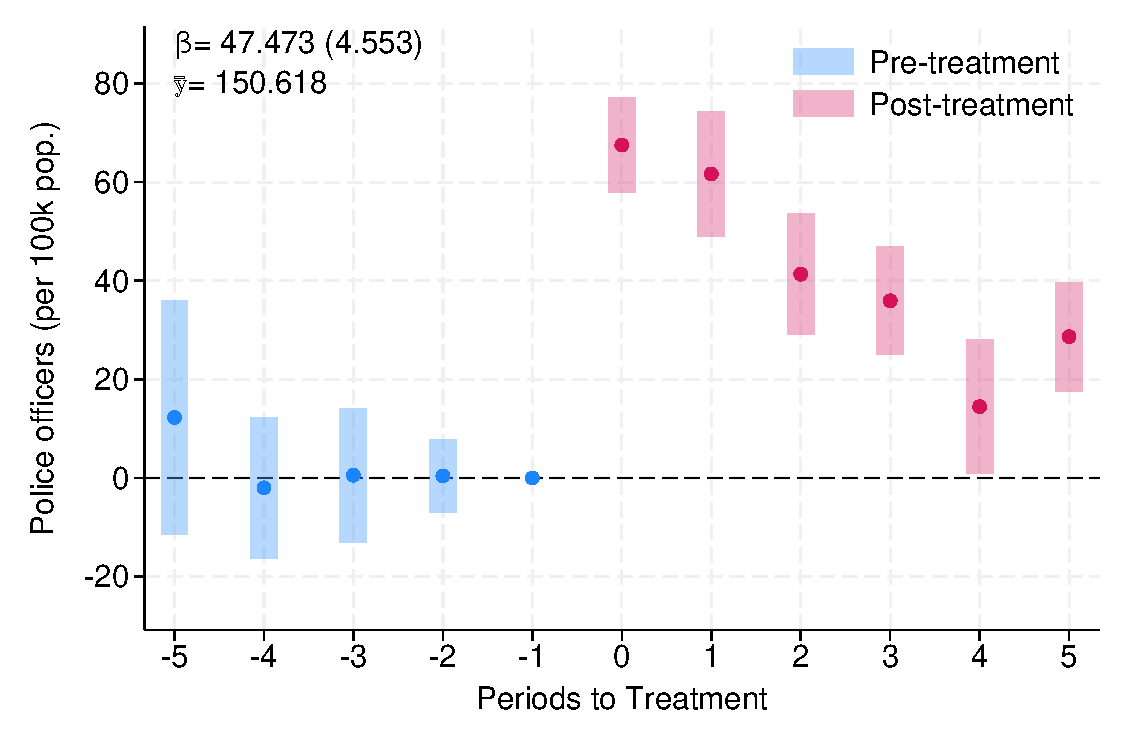
\includegraphics[width=\linewidth]{../manuscript/Graphs/fig4_officers.pdf}

            \small (a) Effect on the number of police officers
        \end{minipage}
        &
        \begin{minipage}[t]{0.48\textwidth}
            \centering
            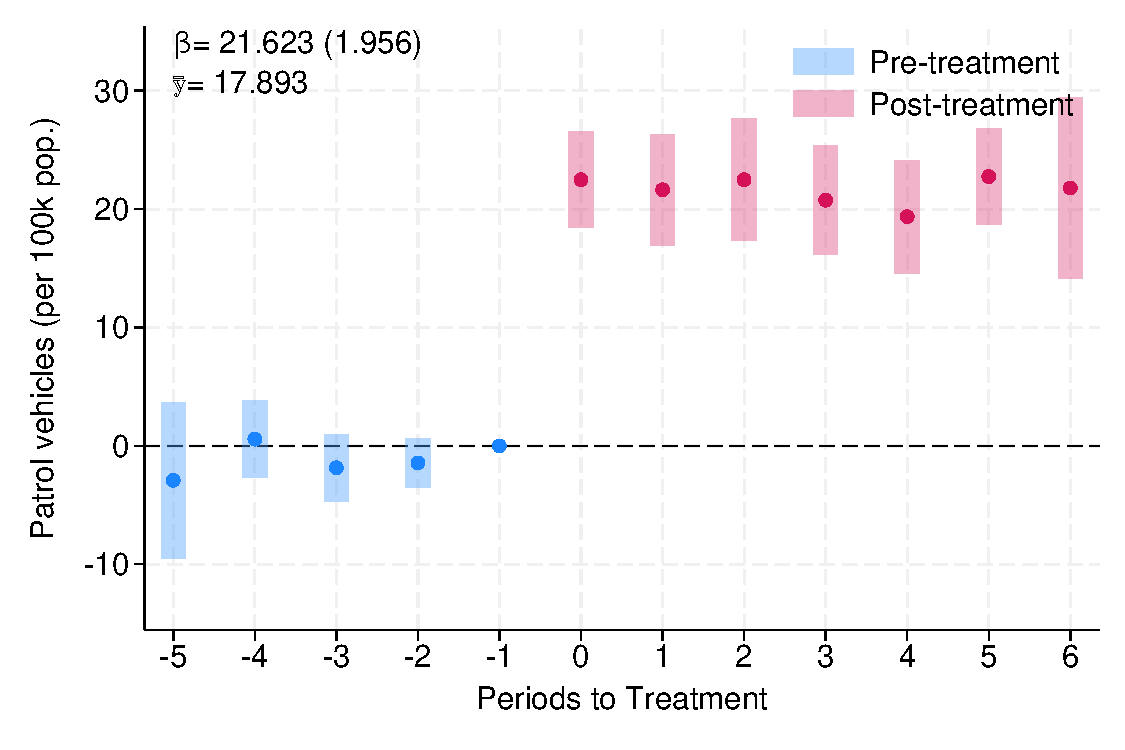
\includegraphics[width=\linewidth]{../manuscript/Graphs/fig4_patrols.pdf}

            \small (b) Effect on the number of patrol vehicles
        \end{minipage}
        \\[4pt]
        \begin{minipage}[t]{0.48\textwidth}
            \centering
            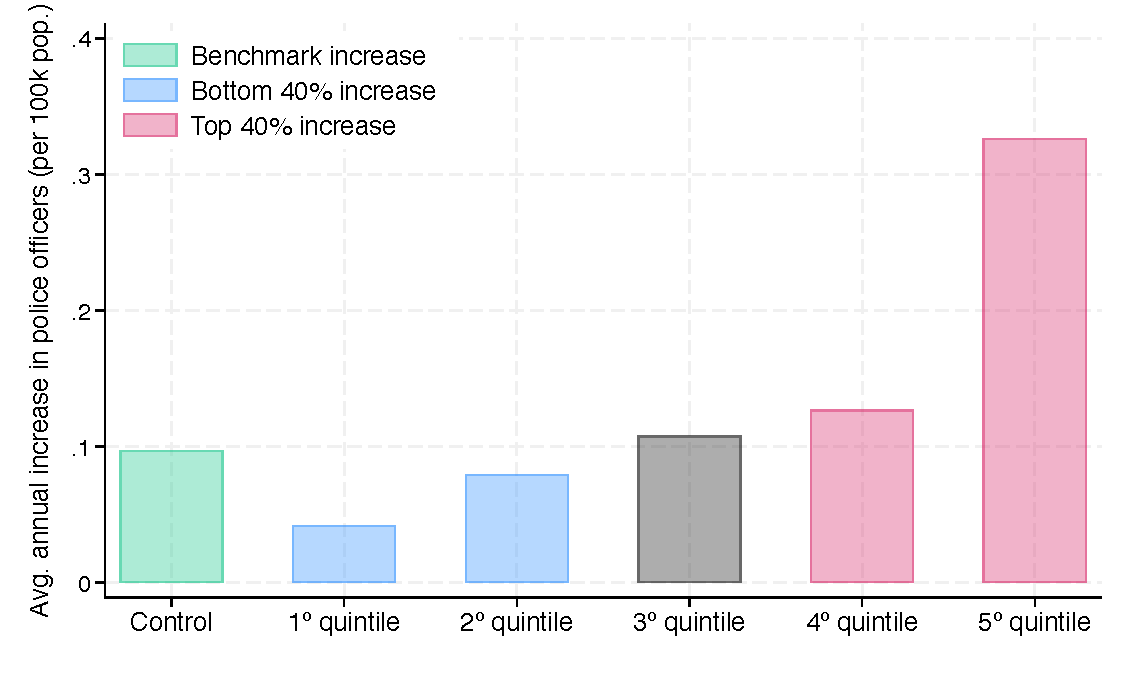
\includegraphics[width=\linewidth]{../manuscript/Graphs/increase_enusc_off_quintiles.pdf}

            \small (c) Distribution of $\Delta$ in police officers
        \end{minipage}
        &
        \begin{minipage}[t]{0.48\textwidth}
            \centering
            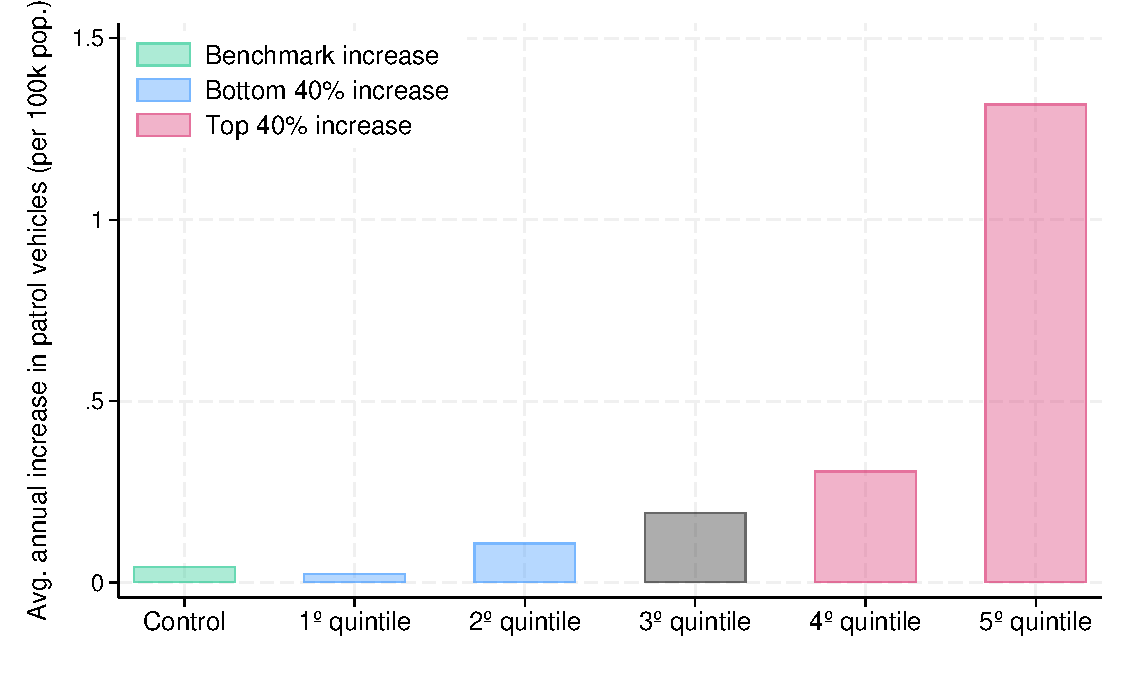
\includegraphics[width=\linewidth]{../manuscript/Graphs/increase_enusc_pv_quintiles.pdf}

            \small (d) Distribution of $\Delta$ in patrol vehicles
        \end{minipage}
        \\[4pt]
        \begin{minipage}[t]{0.48\textwidth}
            \centering
            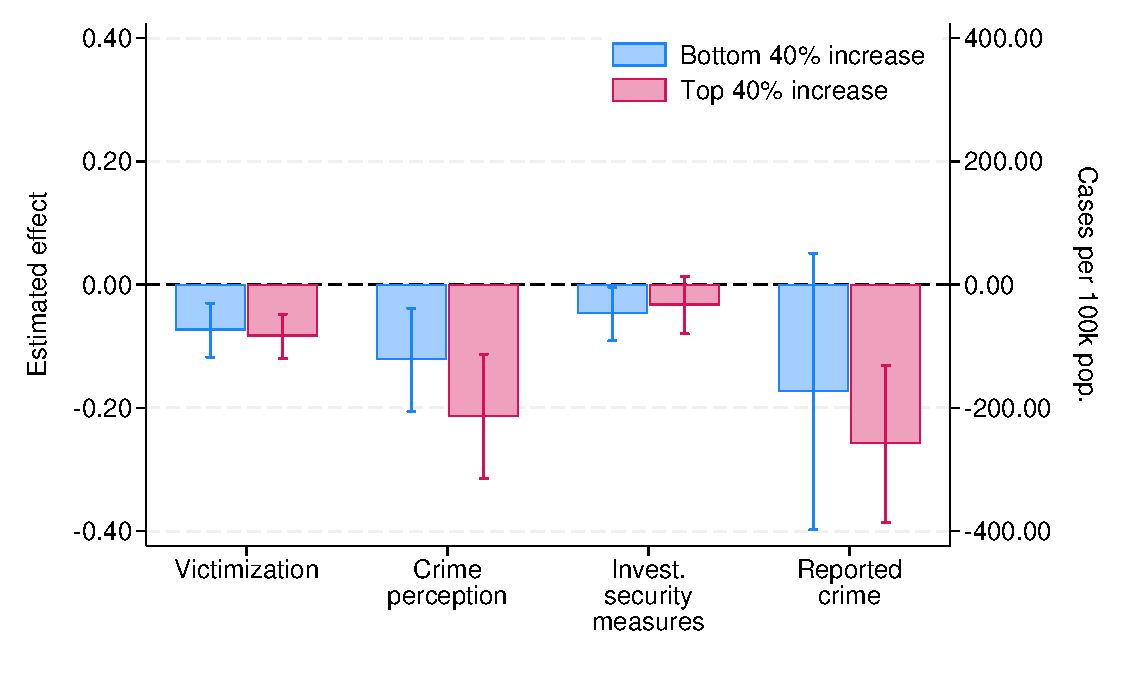
\includegraphics[width=\linewidth]{../manuscript/Graphs/heterogeneity_off.pdf}

            \small (e) Effects by the intensity of $\Delta$ in police officers
        \end{minipage}
        &
        \begin{minipage}[t]{0.48\textwidth}
            \centering
            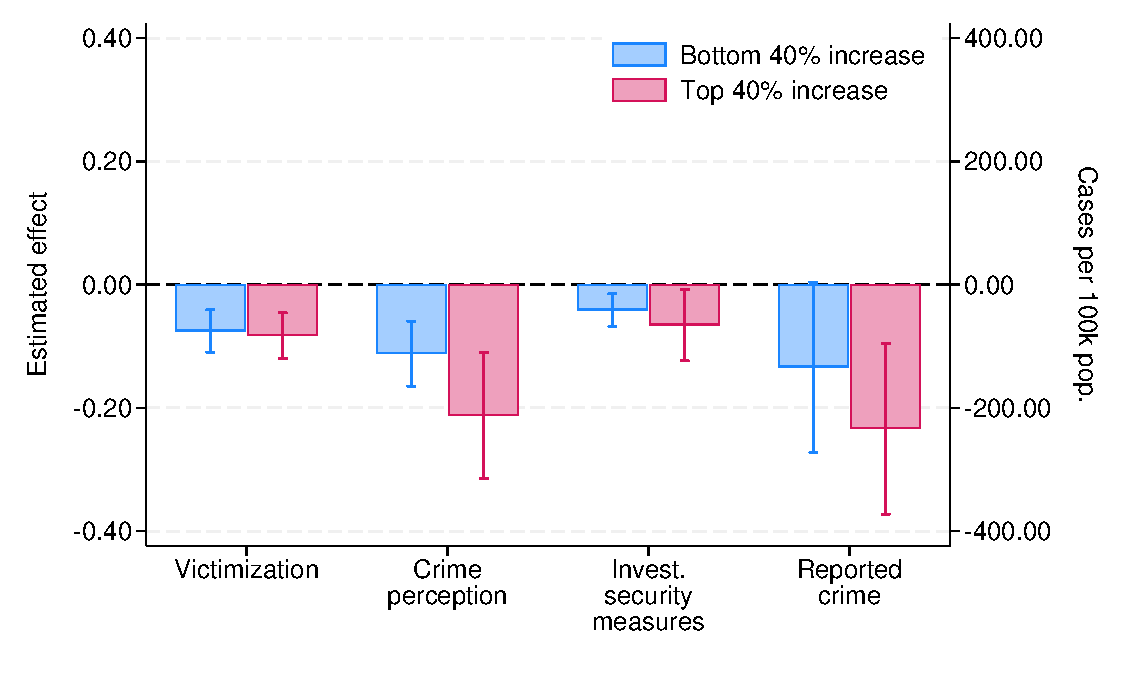
\includegraphics[width=\linewidth]{../manuscript/Graphs/heterogeneity_pv.pdf}

            \small (f) Effects by the intensity of $\Delta$ in patrol vehicles
        \end{minipage}
    \end{tabular}
    \vspace{4pt}
    \begin{minipage}{0.99\textwidth}
    \footnotesize Notes: Panels (a) and (b) show the effect of \emph{Plan Cuadrante} on police officers and patrol vehicles per 100,000 inhabitants. Panels (c) and (d) show the distribution of annual changes in officers and patrol vehicles across municipalities. Panels (e) and (f) report effects by the intensity of resource changes, comparing municipalities in the bottom 40\% and top 40\% of the distribution. The estimation follows \citet{Callaway}. The graphs display estimated coefficients and 95\% confidence intervals. Standard errors are clustered at the municipality level using wild bootstrapping.
    \end{minipage}
\end{figure}
\FloatBarrier
Panels (c) and (d) of Figure \ref{fig:resources} show that the average increase in police resources masks substantial heterogeneity. Municipalities in the bottom 40\% of the resource-change distribution (blue bars) experienced increases close to the average annual variation observed among never treated and not-yet-treated municipalities (green bar). By contrast, municipalities in the top 40\% (red bars) experienced much larger increases, with officers rising by around 22\% and patrol vehicles by around 80\%. If the effects of \emph{Plan Cuadrante} were driven by resource increases alone, we would not expect effects in municipalities whose resource increases were similar to those of the control group. Yet panels (e) and (f) of Figure \ref{fig:resources} show sizeable effects for most crime and crime-perception outcomes even in that low-increase group. While there may be a resource gradient for some crime-perception outcomes, the effects on twelve-month victimization and private investment in security among municipalities with control-like resource increases are close in magnitude to those in municipalities with larger increases. Reassuringly, municipalities in the top and bottom 40\% of the resource-increase distribution do not display differential pre-treatment trends in outcomes or police resources, which suggests that this heterogeneity is not driven by differential pre-existing trends.\footnote{We test for the joint significance of the pre-treatment coefficients between the two groups, separately for the split based on the increase in police officers and the split based on the increase in patrol vehicles. The resulting p-values are, respectively, 0.823 and 0.048 for victimization, 0.059 and 0.379 for crime perception, 0.820 and 0.157 for investment in security measures, and 0.213 and 0.419 for reported crime, as well as 0.616 and 0.444 for police officers and 0.405 and 0.157 for patrol vehicles.}

Although we cannot fully separate the beat policing component from the resource component of the reform---resources may have been important to enable effective implementation of the program, or may explain part of the effects in some municipalities---the fact that municipalities with resource increases similar to those experienced by control municipalities still display sizeable effects indicates that the effects of \emph{Plan Cuadrante} are not driven entirely by resources.\footnote{We also re-estimate the results in Figure \ref{fig:figure02} but controlling for police resources. Online Appendix Table \ref{tab:results_controlbyresources} shows that the magnitude of the estimated effects remains similar for most variables, although the statistical significance is reduced in some estimations. This likely reflects a mechanical feature of the \citet{Callaway} estimation procedure: control variables are not incorporated parametrically, but are instead used to construct the comparison group via outcome regression or propensity-score weighting, so the resulting estimation uncertainty propagates to the ATT standard errors. Note, in addition, that police resources are a bad control---i.e., at least part of their variation is a result of the adoption of \emph{Plan Cuadrante}---so these results should be interpreted cautiously.}\footnote{Table \ref{tab:resourcecorrelates} in Online Appendix \ref{sec:appendixB} examines which factors are associated with a larger increase in police resources upon the adoption of \emph{Plan Cuadrante}.}


\FloatBarrier
%--- Implementation
\begin{figure}[h!]
    \centering
    \caption{Police Resources and Public Safety}
    \label{fig:resources2}
    \begin{subfigure}[t]{0.55\textwidth}
        \centering
        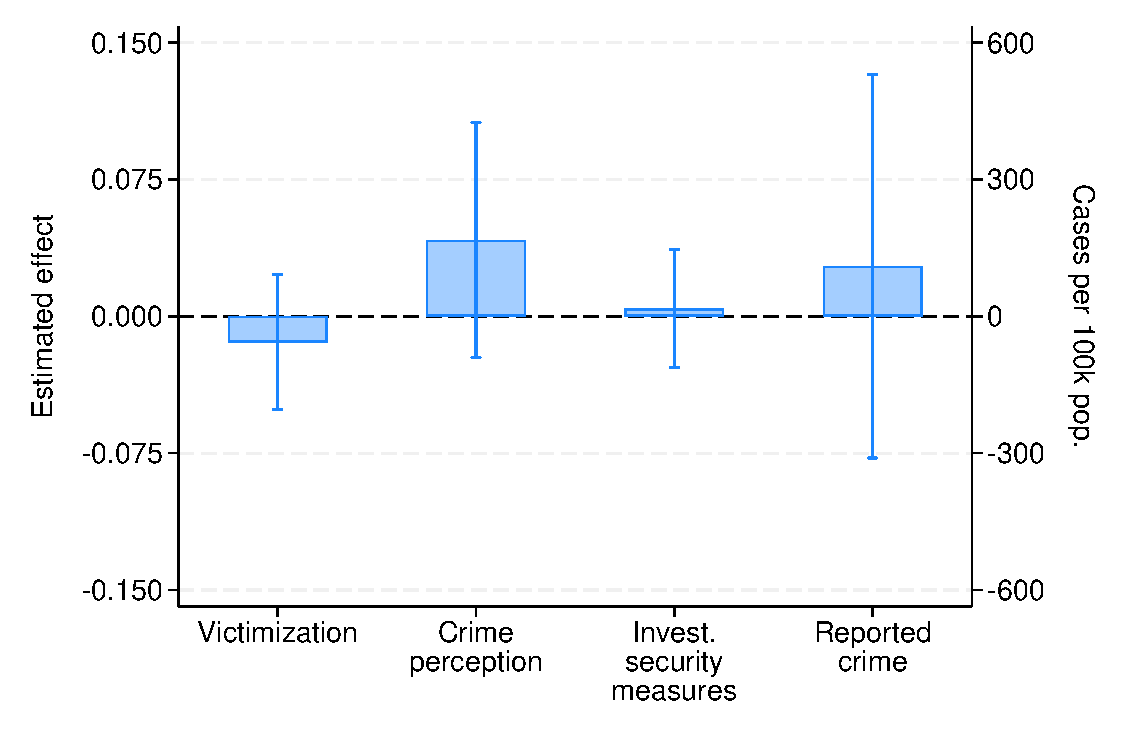
\includegraphics[width=\linewidth]{../manuscript/Graphs/results_SC_att_combined.pdf}
        \caption{Effects of \emph{Seguridad Ciudadana}}
    \end{subfigure}
    \\[6pt]
    \begin{subfigure}[t]{0.55\textwidth}
        \centering
        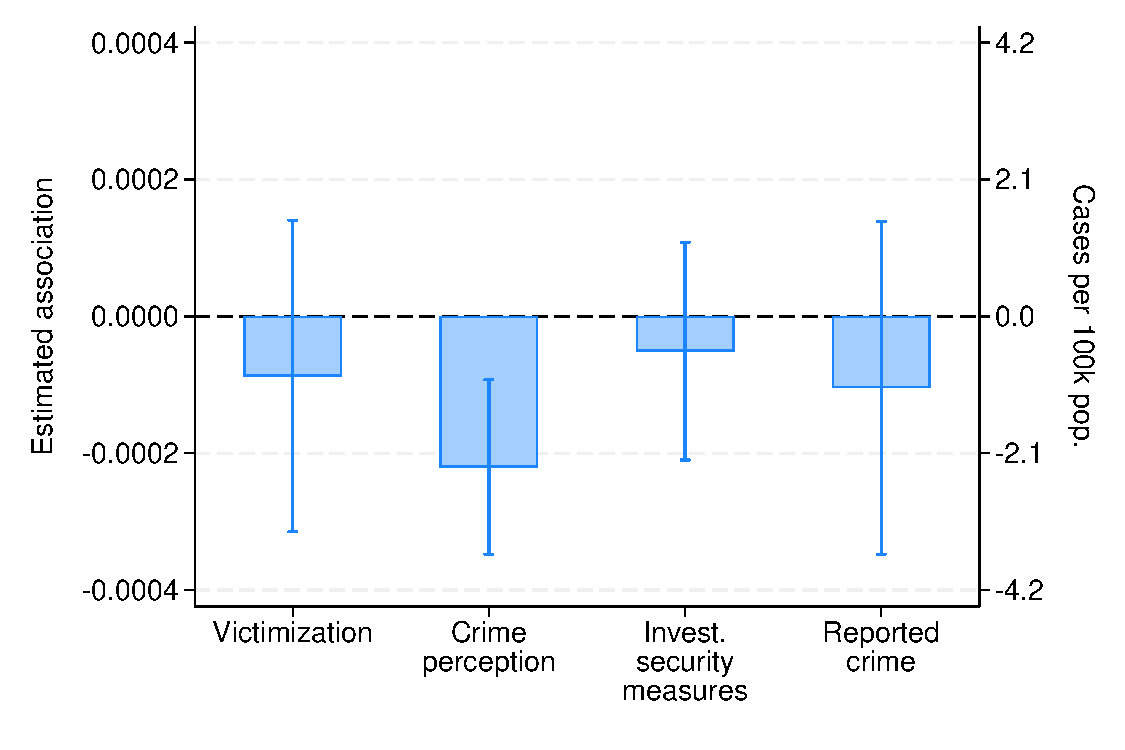
\includegraphics[width=\linewidth]{../manuscript/Graphs/results_corr_novariation_off_santiago.pdf}
        \caption{Association between police officers and effectiveness}
    \end{subfigure}
    \\[6pt]
    \begin{subfigure}[t]{0.55\textwidth}
        \centering
        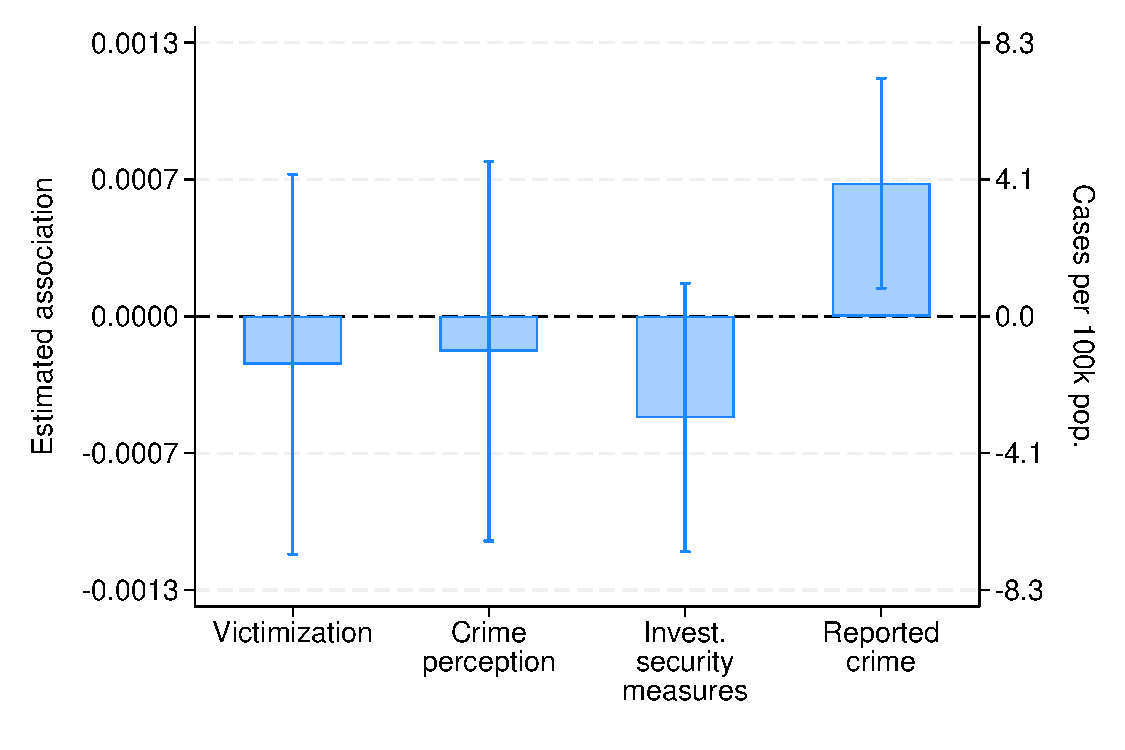
\includegraphics[width=\linewidth]{../manuscript/Graphs/results_corr_novariation_veh_santiago.pdf}
        \caption{Association between patrol vehicles and effectiveness}
    \end{subfigure}
    \\[8pt]
    \begin{minipage}{0.99\textwidth}
    \footnotesize Notes: Panel (a) reports the pooled effect of \emph{Seguridad Ciudadana}, a program that expanded local security personnel to support patrolling and deterrence but did not replicate the deployment-and-strategy features of \emph{Plan Cuadrante}. Panels (b) and (c) report within-municipality associations between police resources and police-effectiveness outcomes among the 41 municipalities of the Santiago Metropolitan Region, all of which had adopted \emph{Plan Cuadrante} by 2000. The regressions include municipality and year fixed effects. Standard errors are clustered at the municipality level using the wild bootstrapping procedure.
    \end{minipage}
\end{figure}
\FloatBarrier

To further investigate whether resource increases alone can explain our results, we assess the effects of \emph{Seguridad Ciudadana}, a program that expanded local security personnel to support patrolling and deterrence, but did not replicate the core deployment-and-strategy features of \emph{Plan Cuadrante}. Using a difference-in-differences specification following \citet{Callaway}, panel (a) of Figure \ref{fig:resources2} shows no significant effects of these resource changes on police effectiveness. Further details about this exercise and the corresponding event-study estimates are reported in Online Appendix \ref{sec:appendixB} and Online Appendix Figure \ref{fig:figureA5}. 


Finally, we study whether variation in police resources in municipalities that had already adopted \emph{Plan Cuadrante} improves public safety and security perceptions. Using ENUSC data and information on resources for 2006--2012 in the 41 municipalities of the Santiago Metropolitan Region---all of which had adopted \emph{Plan Cuadrante} by 2000---we exploit variation in officers and patrol vehicles that is unrelated to program adoption. Panels (b) and (c) of Figure \ref{fig:resources2} show the association between police resources and our main outcomes, conditional on municipality and year fixed effects. With one exception---the association between police officers and crime perception---none of these associations is statistically significant at conventional confidence levels. \footnote{Online Appendix Figure \ref{fig:figureA7B} reports the same exercise and also shows similar results for the broader set of municipalities that adopted \emph{Plan Cuadrante} before 2006 and never-treated municipalities (red bars); see Online Appendix \ref{sec:appendixB} for further details.}

Taken together, these results suggest that resource increases alone do not account for the effects of \emph{Plan Cuadrante}. We next turn to evidence that speaks more directly to the beat-policing components of the reform.

Panel (a) of Figure \ref{fig:police_performance} shows that, following the adoption of \emph{Plan Cuadrante}, households are much more likely to report increased police presence in their neighborhoods. The share of households perceiving increased police presence rises by 35 percentage points (156\%), the share reporting that police pass by their house daily rises by 22 percentage points (59\%), the share reporting never seeing police patrols near their house falls by 10 percentage points (57\%), and complaints about lack of police surveillance fall by around 5 percentage points (20\%). This evidence is consistent with both larger resources and the new deployment model. Yet the latter estimate---the only police-presence outcome for which we can separately estimate effects in municipalities with small and large resource increases---is similar in magnitude across the two groups, which suggests that the increase in police presence is not explained only by larger resource increases (see Online Appendix Figure \ref{fig:heterogeneity_appendix}).\footnote{We cannot estimate heterogeneous effects for other police-presence outcomes, such as the reporting of police passing by or the share of households perceiving an increase in police presence, because those variables are available only in ENUSC rounds 2003, 2005, and 2006, while resource data start in 2006.} More importantly, the broader pattern of results suggests that \emph{Plan Cuadrante} did more than simply increase patrolling intensity. Existing work shows that police presence can reduce crime while officers are present, but that its overall effects may be attenuated when crime is displaced across places or time windows \citep{MASTROBUONI2019, Blanes_Mastrobuoni_2018}. Our results point to something broader. As discussed in Section \ref{results}, we find actual declines in victimization and reported crime, together with no evidence of spillovers to neighboring municipalities. This pattern is more consistent with officers accumulating local knowledge and adapting prevention strategies to local conditions under stable territorial assignment than with a purely mechanical increase in patrol intensity.

Panel (b) of Figure \ref{fig:police_performance} reinforces this interpretation. Households in early-adopting municipalities report better police performance across multiple dimensions. They are 8.1 percentage points (16\%) more likely to rate police performance as good or very good, 7.6 percentage points (11\%) more likely to describe police as efficient, 5 percentage points (6\%) more likely to report that police are helpful, and 4.9 percentage points (7\%) more likely to report that police are well informed. They are also 3.9 percentage points (10\%) less likely to perceive police as corrupt, 7.9 percentage points (21\%) less likely to believe police fail to control crime, and 7.6 percentage points (22\%) less likely to report that police do not perform their duties effectively.\footnote{Information on police performance is only available in ENUSC round 2005. Using this round, we compare perceived police performance in municipalities that adopted \emph{Plan Cuadrante} in 2005 or earlier and in municipalities adopting after 2005. Figure \ref{fig:balance_doseresponse} in Online Appendix \ref{sec:appendixB} shows that the number of years of exposure to \emph{Plan Cuadrante} is positively correlated with perceived police performance. While these exercises on perceived police performance should be interpreted with caution, we show in the same appendix that the timing of future adoption is not correlated with perceived police performance in 2005 for municipalities that had not yet adopted the program by 2005.} %These perceived improvements are consistent with a setting in which officers become better informed about local routines and more effective in how they patrol and respond.

The administrative evidence points in the same direction. Panel (c) of Figure \ref{fig:police_performance} shows that arrests per 100,000 inhabitants increase by 48 (14\%) in our main estimates, even as crime declines overall.\footnote{As with reported crime, this event study is restricted to 5 pre-treatment and 7 post-treatment periods for symmetry with the ENUSC-based analysis; Online Appendix Figure \ref{fig:admin_uncapped} reports the results for arrests using the full set of pre-treatment and post-treatment periods.} This effect is also significant among municipalities with resource increases similar to those in the control group (see Online Appendix Figure \ref{fig:heterogeneity_appendix}). Consistent with this pattern, panel (d) of Figure \ref{fig:police_performance} shows that the arrest rate per reported crime also increases by 1.7 percentage points (10\%), suggesting that a higher share of crimes reported to the police are being solved. Because these gains appear even where resources did not increase more than in control municipalities, they are difficult to reconcile with a pure resource story and are more naturally interpreted as improvements in police effectiveness under the deployment and strategy changes introduced by \emph{Plan Cuadrante}. The corresponding event-study estimates for arrests, the arrest rate per reported crime, and trust in the police in Figure \ref{fig:police_performance} confirm that these changes emerge only after adoption.

Finally, panel (e) of Figure \ref{fig:police_performance} shows a sharp increase in trust in the police in our main specification (Section \ref{results}), consistent with one of the objectives of beat policing, namely bringing officers closer to the community and allowing them to accumulate local knowledge through repeated interaction. Online Appendix Figure \ref{fig:heterogeneity_appendix} shows that this effect remains sizeable both in municipalities that experienced resource increases similar to the control group and in those with larger increases.

Overall, although resources were likely important for implementation and may explain part of the effects in some municipalities, the results in this section indicate that resource changes alone are not enough to explain our findings. The evidence is more consistent with a combination of deployment changes and the strategy adjustments enabled by local knowledge accumulation under permanent assignment to quadrants.

\FloatBarrier
%--- Implementation
\begin{figure}[!ht]
    \centering
    \caption[\emph{Plan Cuadrante} and Changes in Police Performance]{\emph{Plan Cuadrante} and Changes in Police Performance}
    \label{fig:figure05}
    \label{fig:police_performance}
    \label{fig:effectiveness_es}
    \begin{subfigure}[t]{0.44\textwidth}
        \centering
        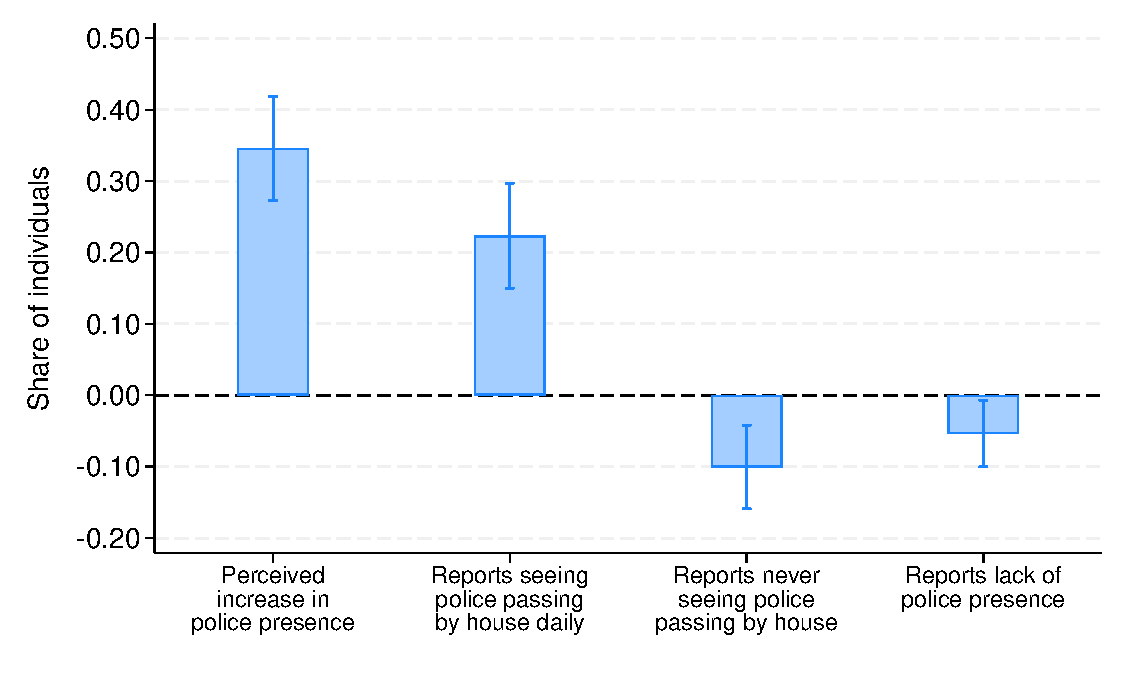
\includegraphics[width=\linewidth]{../manuscript/Graphs/results_policepresence.pdf}
        \caption{Effect on police presence}
    \end{subfigure}\hfill
    \begin{subfigure}[t]{0.44\textwidth}
        \centering
        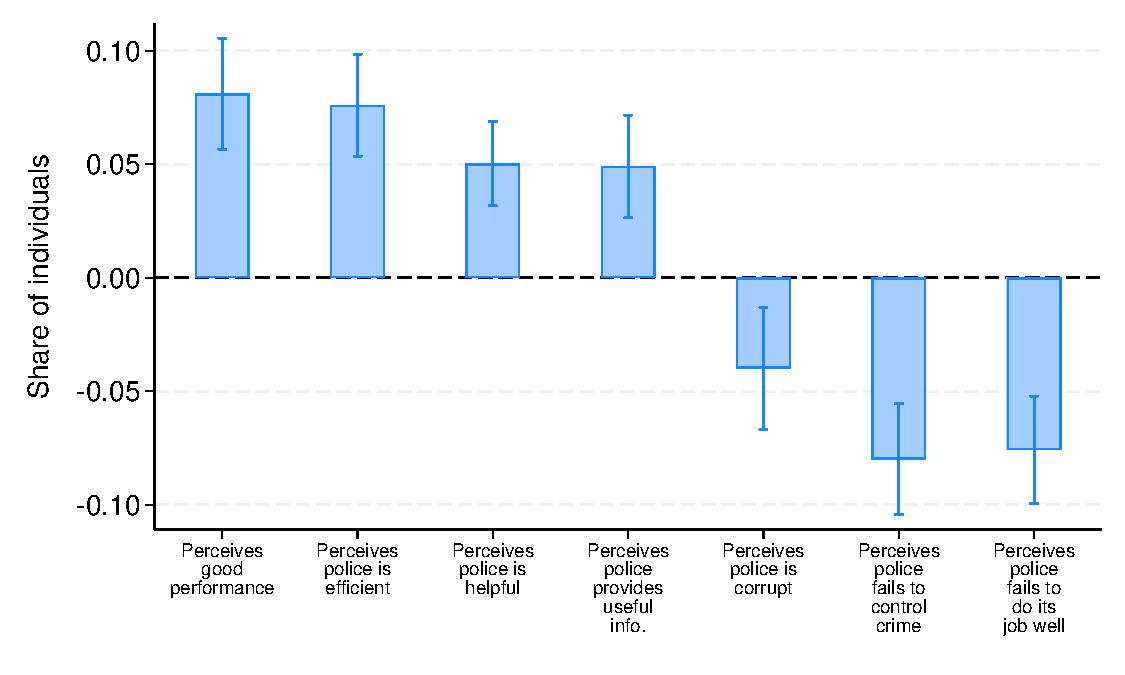
\includegraphics[width=\linewidth]{../manuscript/Graphs/combined_PCttest_2.pdf}
        \caption{Effect on perceived police performance}
    \end{subfigure}
    \\[6pt]
    \begin{subfigure}[t]{0.44\textwidth}
        \centering
        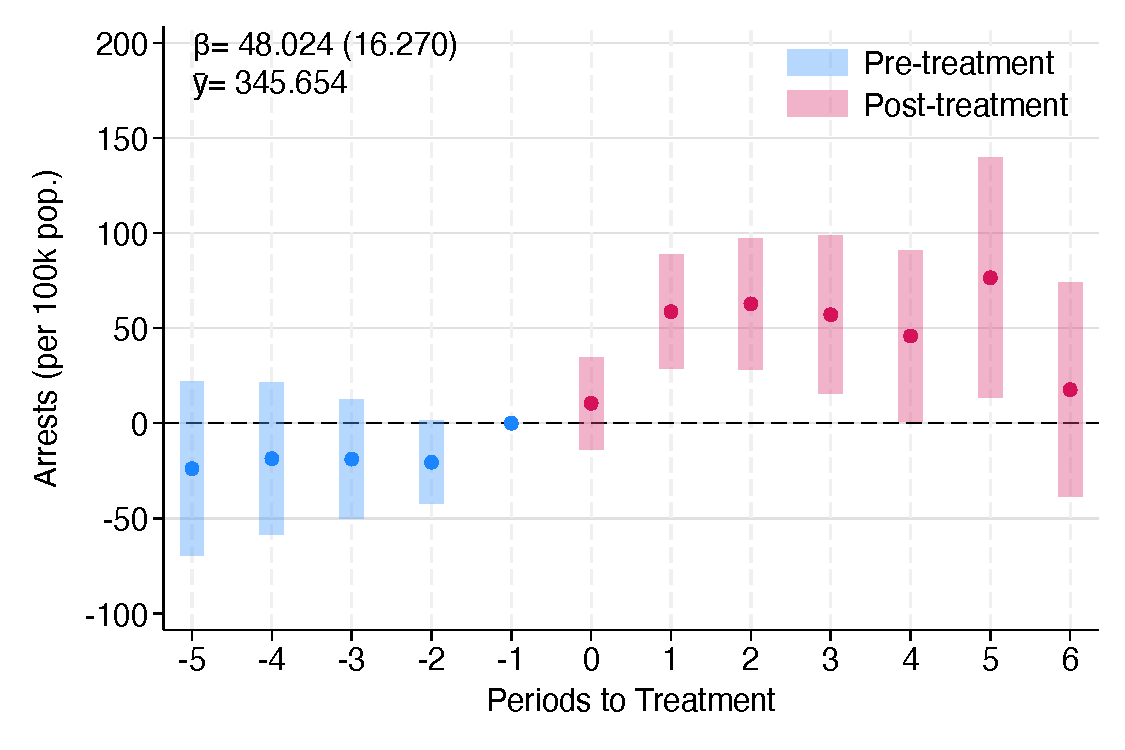
\includegraphics[width=\linewidth]{../manuscript/Graphs/totalarrestscrime_allcomunas.pdf}
        \caption{Arrests (per 100k pop.)}
    \end{subfigure}\hfill
    \begin{subfigure}[t]{0.44\textwidth}
        \centering
        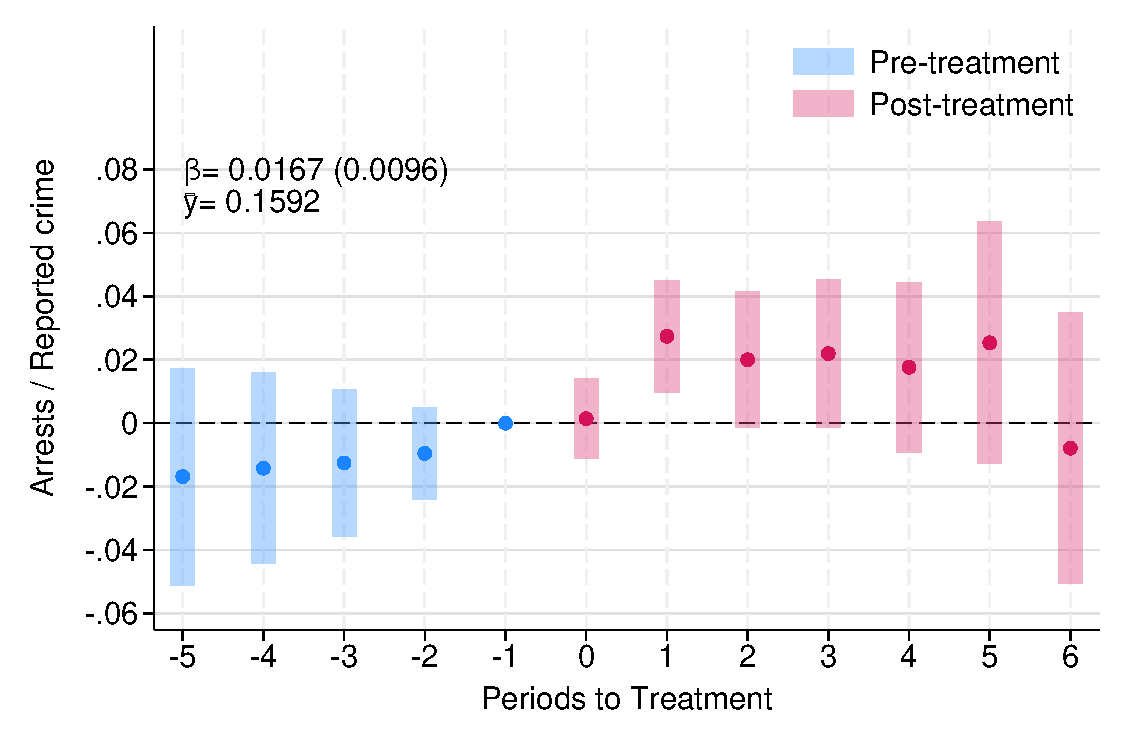
\includegraphics[width=\linewidth]{../manuscript/Graphs/arrests_over_reportedcrime_allcomunas.pdf}
        \caption{Arrests / Reported crime}
    \end{subfigure}
    \\[6pt]
    \begin{subfigure}[t]{0.44\textwidth}
        \centering
        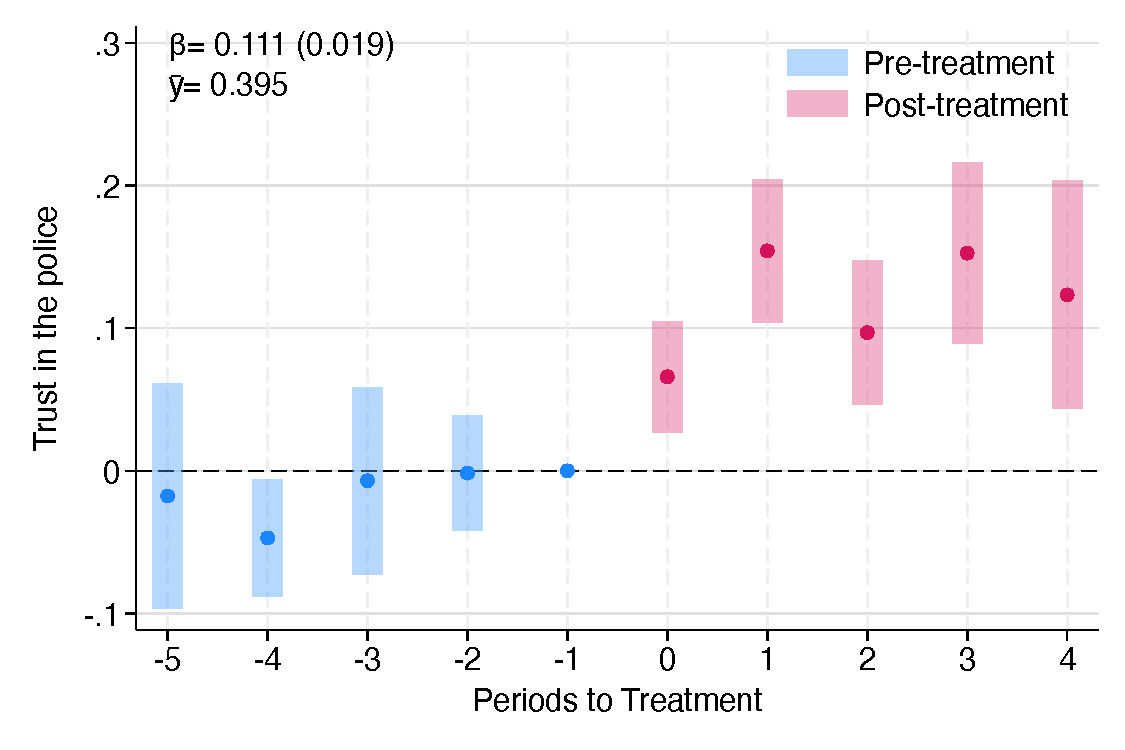
\includegraphics[width=\linewidth]{../manuscript/Graphs/results_trustcarabineros.pdf}
        \caption{Trust in the police}
    \end{subfigure}
    \\[8pt]
    \begin{minipage}{0.99\textwidth}
    \footnotesize Notes: Panel (a) reports the effects on perceived police presence. Panel (b) reports perceived police performance in 2005, comparing municipalities where \emph{Plan Cuadrante} was already implemented before 2006 with municipalities where it was implemented after 2005. Panels (c), (d), and (e) report dynamic event-study estimates for arrests per 100,000 inhabitants, the ratio of arrests to reported crime, and trust in the police. The estimation follows \citet{Callaway}. The graphs display estimated coefficients and 95\% confidence intervals. Standard errors are clustered at the municipality level using the wild bootstrapping procedure.
    \end{minipage}
\end{figure}

\FloatBarrier

%Overall, while resources were arguably important for implementation, the evidence suggests that the beat policing elements---permanent assignment of officers to quadrants and greater local knowledge---were important drivers of the improvements in public safety and security perceptions we document in the paper.



 


% Dani, necesitamos crear dos figuras nuevas combinando parte de los resultados que ya tenemos. 

%% Figure 4: \emph{Plan Cuadrante} and Changes in Police Presence and Resources 
% Panel (a) - Differences in perceptions of police between early and late adopters: 
% Variables to include: 
% Very good/good performance of the police; police is efficient; police is helpful; police provides useful information; police is corrupt; police fails to control crime, police fails to do its job well. Please check well the questions in the survey and define labels with a structure as: "Reports ... " "Perceives ...".
% y-axis: Share of households
% x-axis: Label of the question 

% Panel (b) -  Effect in police presence 
% Bars with diff-in-diff estimates of "Perceived increase in police presence", "Reports seeing police passing by their house daily", "Reports never seeing police passing by their house", "Complaints about lack of police presence"
% y-axis: Share of households 
% x-axis: Periods to treatment

% Panel (c) - Effect in the number of Police Officers
% y-axis: Police officers per 100k inhabitants
% x-axis: Periods to treatment

% Panel (d) - Effect in the number of Police Patrols
% y-axis: Police patrols per 100k inhabitants
% x-axis: Periods to treatment


%% Figure 5: Police Resources and Police Effectiveness

% Panel (a) Distribution of Delta in Police Officers
% Panel (b) Distribution of Delta in Police Patrols 
% Panel (c) Effects by the Intensity of Delta in Police Officers (add bars on "Complaints about lack of police officers")
% Panel (d) Effects by the Intensity of Delta in Police Officers (add bars on "Complaints about lack of police officers")
% Panel (e) Summarize figure A6 in a single panel. One bar per outcome summarizing diff-in-diff estimate. 
% Panel (f) Summarize figure A5 in a single panel. Put ENUSC and admin data together using two y-axis. Combine results for delta officers and delta patrols using different colors for each of them. 

